\chapter{Method}\label{chapter:first_real_chapter}

Our method is based on an Hiearchical VAE (H-VAE), as these have been shown to improve the sharpness of the resulting generated sample\cite{vahdat2020nvae}. There are 3 submodels present, the image encoder $p_\theta(x | z)$\footnote[1]{$z$ will consist of multiple layers as it is an H-VAE. Sometimes denoted as $z_{1:L}$.}, the image decoder $q_\phi(z | x)$\footnotemark[1] and the label decoder $q_\xi(z | y)$\footnotemark[1]. The image encoder and decoder can be pretrained on unlabeled data. Subsequently the label decoder will be trained from the (variational) latent variables, on a subset of the inital dataset $\mathcal{D}$.

\begin{figure}[h]
    \begin{minipage}{0.45\textwidth}
        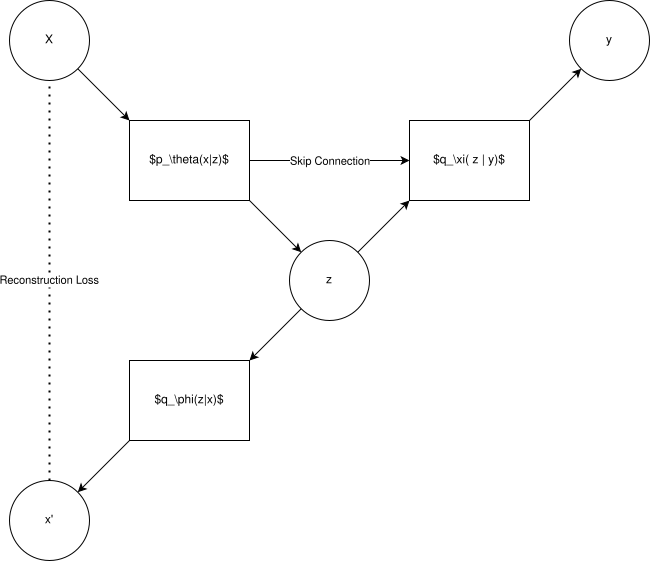
\includegraphics[width=1\textwidth]{figures/model_data_flow.png}
        \caption{The data flow of the various submodels.}
    \end{minipage}
    \hfill
    \begin{minipage}{0.45\textwidth}
        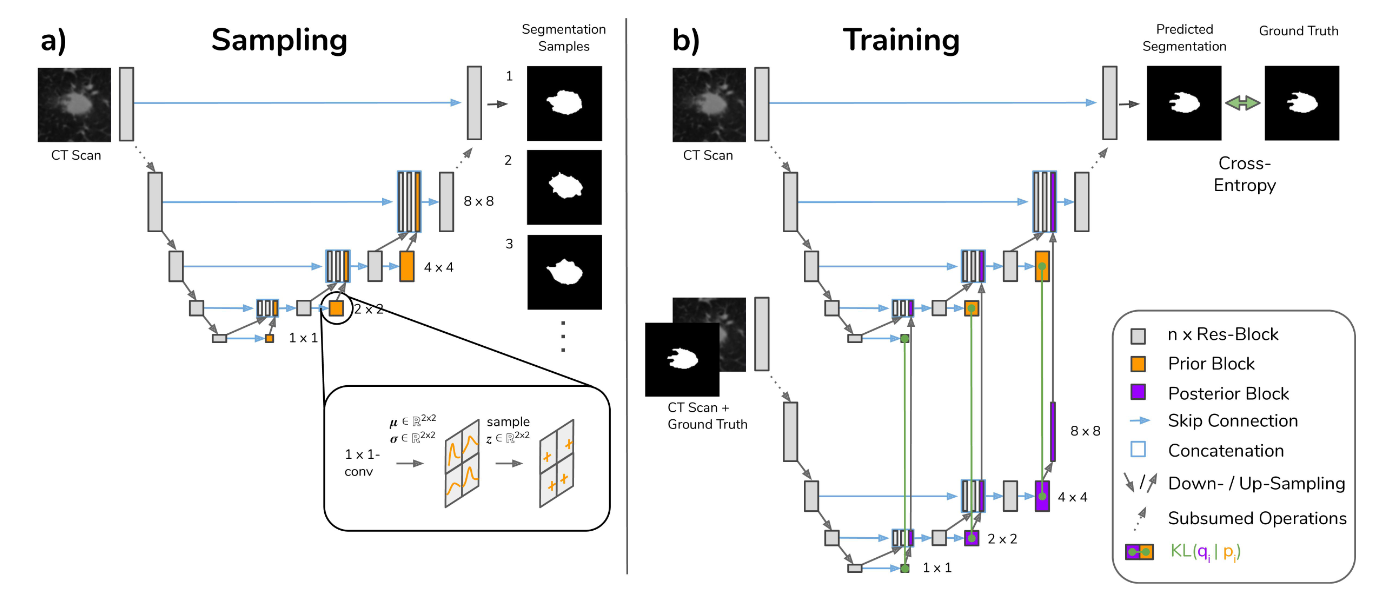
\includegraphics[width=1\textwidth]{figures/h_vae_structure.png}
        \caption{Example of the H-VAE structure. From \cite{kohl2018probabilistic}. This does not include the pretraining of the encoder.}
    \end{minipage}
\end{figure}

\section{Training procedure}
\subsection{Pretraining}
First the model is trained as a VAE, in which the unlabeled (full) dataset is used. Various backbones will be tried, however these will be part of the "ablation" study. Currently three backbones are on my radar:
\begin{itemize}
    \item Resnet50 \cite{he2015deep}
    \item VGG16 \cite{simonyan2015deep}
    \item Vision Transformer \cite{dosovitskiy2021image}
\end{itemize}
The dataset used during pretraining can be indepently chosen compared to the finetuning stage. It can either be the same dataset as the finetuning stage, or a more generic, and thus bigger, dataset. 

\subsection{Fine-Tuning}
The second stage will replace the last layer with a new convolutional layer, as it structure changes. The rest of the model will remain structurly the same. The following choices need to be made, and will be done so after experimentation:
\begin{itemize}
    \item How many of the layers do we copy from the VAE?
    \item How many of the layers do we freeze?
\end{itemize}

% \subsection*{Why VAE?}
% By using a VAE bootstrapping can be applied during inference to provide an insight in the certainty of the model, as has been shown by \cite{kohl2018probabilistic}. This certainty estimation from the bootstrapping is crucial in mobile robotics and can be done quickly using batched inference.

\subsection{Loss functions}
Standard loss function for the H-VAE

\begin{equation}
    \lambda_{HVAE}(x) := \EX_{q(z|x)}[log(p(x|z))] - KL(q(z_1|x)||p(z_1)) - \sum_{l=2}^{L} \EX_{q(z_{<l} | x)}[q(z_l| x, z_{<l}) ||p(z_l|z_{<l})]
\end{equation}


Loss function for the Hierarchical Variational Segmenter
\begin{equation}
    f_{\theta, \xi}(x) = p_\theta()
\end{equation}
\begin{equation}
    \lambda_{HVS}(x, y) := CELoss(f_{\theta, \xi}(x), y) - KL(q(z_1|x)||p(z_1)) - \sum_{l=2}^{L} \EX_{q(z_{<l} | x)}[q(z_l| x, z_{<l}) ||p(z_l|z_{<l})]
\end{equation}

\section{Evaluation}

\subsection{Inference}
Due to the variational architecture of the model, the inference can be done either deterministic, by taking the mean of each latent vector. Or variational, by sampling each latent vector. The benefit of sampling is that there is a possibility to use bootstrapping to get an estimate of the uncertainty. Kohl et al. \cite{kohl2018probabilistic} have shown that bootstrapping can be used to produce an uncertainty measure in neural networks. Furthermore, bootstrapping allows for an ensemble which might improve the top-1 accuracy of the model.


\subsection{Metrics}
Within classification the most well-known and widely used metrics are precision (\ref{eq:precision}), recall (\ref{eq:recall}), and F1-score (\ref{eq:f1})\cite{rijsbergen1979information}. Of which the latter is a combination of precision and recall. Within the field of image segmentation, the F1-score is also Sometimes refered to as the Recognition Quality (RQ)
\begin{equation}
    \label{eq:precision}
    \text{Precision} = \frac{TP}{TP + FP}
\end{equation}
\begin{equation}
    \label{eq:recall}
    \text{Recall} = \frac{TP}{TP + FN}
\end{equation}
\begin{equation}
    \label{eq:f1}
    F1 = \text{RQ} = 2 \cdot \frac{\text{Precision} \cdot \text{Recall}}{\text{Precision} + \text{Recall}}
\end{equation}
The Jaccard Index (\ref{eq:jaccard}) is also widely used as it provides a 

\begin{equation}
    \label{eq:jaccard}
    \text{Jaccard Index} = \frac{TP}{TP + FN + FP}
\end{equation}


To determine the quality of the uncertainty estimation produced by bootstrapping, the Expected Callibration Error (ECE), proposed by Naeini et al. \cite{naeini2015obtaining}, will be measured. 

\begin{equation}
    \text{ECE} = \sum_{m=1}^M \frac{|B_m|}{n} \left| \text{acc}(B_m) - \text{conf}(B_m) \right|
\end{equation}
where:
\begin{itemize}
    \item \(M\) is the number of bins.
    \item \(B_m\) is the set of indices of samples whose predicted probabilities fall into the \(m\)-th bin.
    \item \(|B_m|\) is the number of samples in bin \(m\).
    \item \(n\) is the total number of samples.
    \item \(\text{acc}(B_m)\) is the accuracy of the \(m\)-th bin.
    \item \(\text{conf}(B_m)\) is the average confidence of the \(m\)-th bin.
\end{itemize}
